\chapter{A composição química dos seres vivos}\label{ch:g10:chemistry-of-life}

Deixe uma fatia de pão tempo demais na grelha e ela fica preta: o que
sobra é quase só carbono. Pese uma fatia de maçã fresca, seque-a por um
dia num forno morno, pese-a de novo: cinco sextos da massa dela saíram
como vapor de água. Pão, maçã, carvalho, água-viva, você --- todo ser
vivo é construído, lá no fundo, a partir da mesma lista curta de
ingredientes químicos, e essa lista não é a lista de que são feitas as
rochas. Este capítulo desmonta a matéria viva, ingrediente por
ingrediente, e pergunta o que a torna distinta.

\section{Os elementos: os mesmos átomos das rochas, em outras proporções}

\begin{definition}[Composição química da matéria viva]\label{def:g10:chemistry-of-life:composition}
A \emph{composição química}\index{composição química} de uma amostra de
matéria viva é a lista dos elementos químicos que ela contém, com a
fração da massa da amostra que cada um representa. Ela é medida
desmontando quimicamente a amostra --- queimando-a, pesando o que
evapora e o que resta, analisando os gases liberados --- e não olhando
para ela.
\end{definition}

\begin{proposition}[Quatro elementos formam 96\% de um corpo vivo]\label{prop:g10:chemistry-of-life:four}
Em massa, a matéria viva é feita quase inteiramente de quatro
elementos: oxigênio (O), carbono (C), hidrogênio (H) e nitrogênio (N).
No corpo humano eles respondem por cerca de 65\%, 18.5\%, 9.5\% e 3.2\%
da massa --- 96\% juntos. Cálcio, fósforo, potássio, enxofre, sódio,
cloro e magnésio dividem a maior parte dos 4\% restantes, e uma dúzia de
\emph{oligoelementos} (ferro, zinco, iodo, cobre\dots) estão presentes
muito abaixo de 0.1\% e ainda assim são indispensáveis. Os mesmos quatro
elementos dominam numa bactéria, num pé de trigo ou numa baleia, em
proporções parecidas.
\end{proposition}
\admitted

\begin{omfigure}
\begin{tikzpicture}
\begin{axis}[
  ybar, bar width=6pt,
  width=0.92\linewidth, height=6.2cm,
  axis x line=bottom, axis y line=left,
  ymin=0, ymax=75,
  ylabel={\% da massa}, ylabel style={font=\small},
  symbolic x coords={O,C,H,N,Ca,P,Si,Al,Fe},
  xtick=data, tick label style={font=\small},
  enlarge x limits=0.08,
  legend style={at={(0.5,-0.22)}, anchor=north, legend columns=2,
                font=\small, draw=none},
  nodes near coords, nodes near coords style={font=\scriptsize},
  point meta=explicit symbolic,
]
\addplot[fill=omDef!70, draw=omDef] coordinates
  {(O,65) [65] (C,18.5) [18.5] (H,9.5) [9.5] (N,3.2) [3.2] (Ca,1.5) []
   (P,1.0) [1.0] (Si,0.01) [] (Al,0.01) [] (Fe,0.01) []};
\addplot[fill=omProp!70, draw=omProp] coordinates
  {(O,46) [46] (C,0.02) [] (H,0.14) [] (N,0.002) [] (Ca,3.6) [3.6]
   (P,0.1) [] (Si,28) [28] (Al,8.2) [8.2] (Fe,5.6) [5.6]};
\legend{corpo humano, crosta terrestre}
\end{axis}
\end{tikzpicture}

{\small Os mesmos elementos, duas receitas bem diferentes: frações
mássicas dos principais elementos num corpo humano e nas rochas da
crosta terrestre (as barras pequenas não levam rótulo: o cálcio é 1.5\%
de um corpo; o carbono é 0.02\% da crosta, o hidrogênio 0.14\%, o
nitrogênio 0.002\%; silício, alumínio e ferro são apenas traços num
corpo). Carbono, hidrogênio e nitrogênio são abundantes na matéria viva
e raros na rocha; silício, alumínio e ferro fazem o contrário.}
\end{omfigure}

\begin{example}[A matéria viva contra a rocha]\label{ex:g10:chemistry-of-life:crust}
A crosta terrestre também é 46\% oxigênio, mas os elementos seguintes
dela são silício (28\%), alumínio (8\%) e ferro (5.6\%). O carbono
compõe 0.02\% da crosta e o nitrogênio 0.002\%, contra 18.5\% e 3.2\% de
um corpo. Um ser vivo não é, portanto, uma amostra do que o cerca: ele
\emph{concentra} alguns elementos por um fator de mil ou mais. Essa
seleção é a primeira assinatura química da vida.
\end{example}

\begin{remark}[De onde vêm os átomos]\label{rem:g10:chemistry-of-life:origin}
Cada um desses átomos é banal: o carbono dos seus músculos era gás
carbônico do ar antes de uma planta o fixar, o nitrogênio das suas
\omterm{def:g10:chemistry-of-life:families}{proteínas} era nitrogênio do ar antes de bactérias do solo o
capturarem. O que a vida tem de especial não são os átomos, e sim o
modo como eles são montados e as proporções em que são reunidos.
\end{remark}

\section{A água e os sais minerais}

\begin{definition}[Matéria mineral e matéria orgânica]\label{def:g10:chemistry-of-life:mineral-organic}
As moléculas de um ser vivo se dividem em dois grupos. A
\emph{matéria mineral}\index{matéria mineral} é feita de moléculas que
também existem fora dos seres vivos: a água e os
\emph{sais minerais}\index{sais minerais} dissolvidos (íons como
$\mathrm{Na^+}$, $\mathrm{K^+}$, $\mathrm{Ca^{2+}}$, $\mathrm{Cl^-}$,
fosfato e bicarbonato). A \emph{matéria orgânica}\index{matéria orgânica}
é feita de moléculas construídas sobre um esqueleto de átomos de carbono
ligados a hidrogênio e, em geral, a oxigênio e nitrogênio --- moléculas
que, na Terra, só são feitas por seres vivos ou a partir dos restos deles.
\end{definition}

\begin{proposition}[A água é o constituinte principal]\label{prop:g10:chemistry-of-life:water}
A água é a molécula mais abundante de todo ser vivo: cerca de 60\% a
65\% da massa de um adulto humano, 75\% da de um recém-nascido, 85\% da
de uma maçã, 95\% da de uma água-viva, mas apenas 13\% da de um grão de
trigo dormente. O teor de água de uma amostra é medido pesando-a,
secando-a a cerca de \qty{105}{\celsius} até a massa parar de cair, e
pesando-a de novo: a massa perdida é a água.
\end{proposition}
\admitted

\begin{example}[Secando uma fatia de maçã]\label{ex:g10:chemistry-of-life:apple}
Uma fatia de maçã fresca de massa \qty{24.0}{g} é seca até a massa dela
estabilizar em \qty{3.6}{g}. Água perdida: $24.0 - 3.6 = \qty{20.4}{g}$,
ou seja $20.4/24.0 = 0.85$, isto é 85\% da massa fresca. Os
\qty{3.6}{g} que restam são a \emph{matéria seca}: moléculas orgânicas
mais \omterm{def:g10:chemistry-of-life:mineral-organic}{sais minerais}. Queime essa matéria seca e sobrevivem cerca de
\qty{0.1}{g} de cinza clara --- os \omterm{def:g10:chemistry-of-life:mineral-organic}{sais minerais}; o resto, a parte
orgânica, saiu como gás carbônico e vapor de água.
\end{example}

\begin{omfigure}
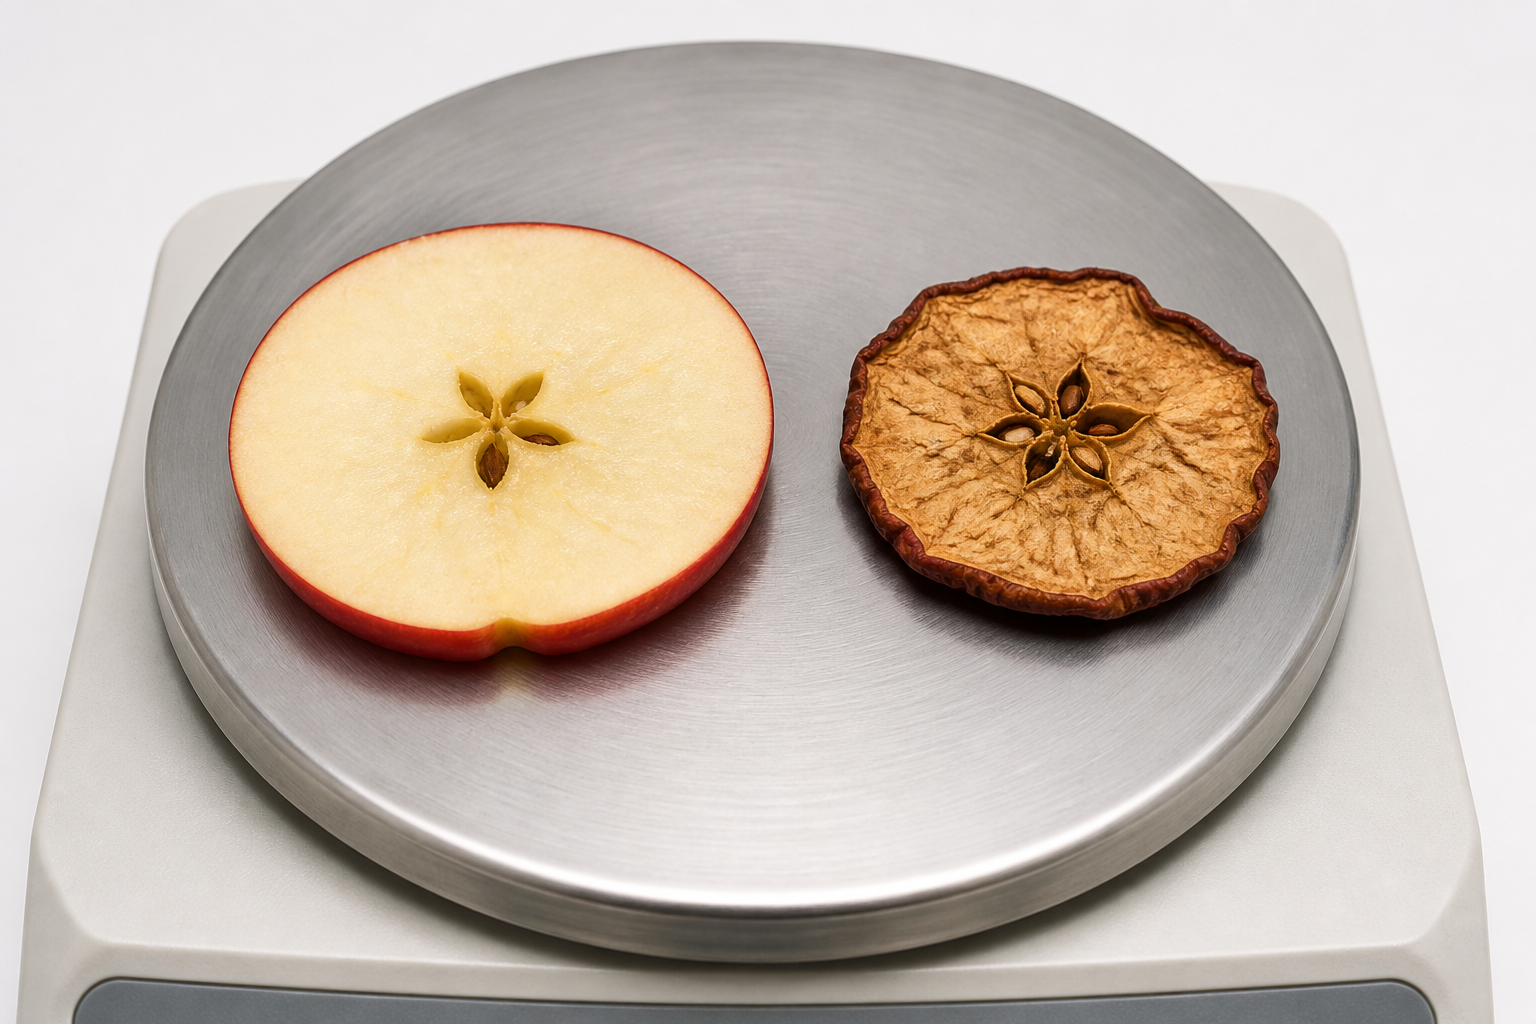
\includegraphics[width=0.56\linewidth]{images/book2/ai/g10-chem-dried-apple.png}

{\small Uma fatia de maçã fresca e a mesma fatia depois de seca: o que
resta é a matéria seca, um sexto da massa inicial. O resto era água.}
\end{omfigure}

\begin{proposition}[O que a água faz]\label{prop:g10:chemistry-of-life:water-roles}
A água é onde a química de uma célula acontece: ela dissolve sais,
açúcares e a maioria das moléculas orgânicas pequenas, de modo que elas
possam se encontrar e reagir; ela as transporta de um lugar para outro
(o plasma sanguíneo é 90\% água, a seiva bem mais); e, porque é preciso
muita energia para aquecê-la, ela amortece a temperatura do organismo
contra mudanças bruscas. Perder 10\% da água do corpo é uma emergência
médica; uma semente dormente, a 13\%, simplesmente desligou a química
dela até a água voltar.
\end{proposition}
\admitted

\begin{example}[Sais minerais que dá para nomear]\label{ex:g10:chemistry-of-life:salts}
O fosfato de cálcio enrijece os ossos e os dentes (o cálcio é 1.5\% da
massa do corpo, quase todo no esqueleto). Os íons sódio e cloreto
fixam a salinidade do sangue, perto de \qty{9}{g/L}; os íons potássio
estão concentrados dentro das células; o ferro fica no coração da
hemoglobina; o iodo é necessário para fabricar o hormônio da glândula
tireoide. Um sal mineral nunca é fonte de energia, mas um corpo privado
de um deles falha numa tarefa precisa.
\end{example}

\section{As moléculas orgânicas: quatro famílias}

\begin{definition}[Carboidratos, lipídios, proteínas, ácidos nucleicos]\label{def:g10:chemistry-of-life:families}
As moléculas orgânicas pertencem a quatro famílias.
\begin{itemize}
  \item Os \emph{carboidratos}\index{carboidrato} (açúcares) contêm
        apenas carbono, hidrogênio e oxigênio. Os açúcares simples são
        unidades isoladas, como a glicose $\mathrm{C_6H_{12}O_6}$; os
        carboidratos complexos são cadeias de centenas ou milhares de
        unidades de glicose --- amido e celulose nos vegetais,
        glicogênio nos animais.
  \item Os \emph{lipídios}\index{lipídio} (gorduras e óleos) também
        contêm apenas C, H e O, mas com bem menos oxigênio, e não se
        dissolvem em água. Os mais comuns são os triglicerídeos, cada
        um feito de uma molécula de glicerol unida a três longas
        cadeias de ácido graxo.
  \item As \emph{proteínas}\index{proteína} são cadeias de
        \emph{aminoácidos}\index{aminoácido}: vinte tipos de
        aminoácido, todos contendo nitrogênio, ligados numa ordem
        precisa em cadeias de cinquenta a vários milhares de unidades
        que se dobram numa forma definida.
  \item Os \emph{ácidos nucleicos}\index{ácido nucleico} (DNA e RNA)
        são cadeias de nucleotídeos, contendo fósforo além de C, H, O e
        N; eles guardam e transmitem a informação genética, e são o
        assunto do \cref{ch:g10:universal-dna}.
\end{itemize}
\end{definition}

\begin{omfigure}
\begin{tikzpicture}[
  box/.style={draw, rounded corners, minimum height=0.9cm, text width=2.6cm,
              align=center, font=\small},
  fam/.style={draw, fill=#1!12, rounded corners, text width=2.6cm, align=center,
              font=\small\bfseries, minimum height=0.8cm,
              text height=1.6ex, text depth=0.4ex},
  >=Stealth]
  \node[fam=omDef] (c) at (0,0) {carboidratos};
  \node[fam=omProp] (l) at (3.2,0) {lipídios};
  \node[fam=omThm] (p) at (6.4,0) {proteínas};
  \node[fam=omMeth] (n) at (9.6,0) {ácidos nucleicos};
  \node[box] (cu) at (0,-1.7) {unidade: glicose\\ $\mathrm{C_6H_{12}O_6}$};
  \node[box] (lu) at (3.2,-1.7) {unidades: glicerol\\ + ácidos graxos};
  \node[box] (pu) at (6.4,-1.7) {unidades: 20 tipos\\ de aminoácido};
  \node[box] (nu) at (9.6,-1.7) {unidades: 4 tipos\\ de nucleotídeo};
  \node[box] (cp) at (0,-3.6) {amido, glicogênio,\\ celulose};
  \node[box] (lp) at (3.2,-3.6) {triglicerídeos,\\ lipídios de membrana};
  \node[box] (pp) at (6.4,-3.6) {enzimas, fibras,\\ anticorpos};
  \node[box] (np) at (9.6,-3.6) {DNA, RNA};
  \foreach \a/\b in {c/cu, l/lu, p/pu, n/nu} \draw (\a) -- (\b);
  \foreach \a/\b in {cu/cp, lu/lp, pu/pp, nu/np}
    \draw[->] (\a) -- node[right, font=\scriptsize] {cadeia} (\b);
  \node[font=\small, anchor=east] at (-1.6,-1.7) {bloco de construção};
  \node[font=\small, anchor=east] at (-1.6,-3.6) {molécula grande};
\end{tikzpicture}

{\small As quatro famílias de moléculas orgânicas. Cada molécula grande
é uma cadeia de blocos de construção pequenos; a identidade do bloco, e
o modo como a cadeia é arranjada, decidem o que a molécula faz.}
\end{omfigure}

\begin{example}[Lendo um rótulo de alimento]\label{ex:g10:chemistry-of-life:label}
Um rótulo de pão integral traz, por \qty{100}{g}: \omterm{def:g10:chemistry-of-life:families}{carboidratos}
\qty{41}{g} (dos quais açúcares \qty{3}{g}), gorduras \qty{3}{g},
\omterm{def:g10:chemistry-of-life:families}{proteínas} \qty{9}{g}, fibras \qty{7}{g}, sal \qty{1.1}{g}. O resto ---
cerca de \qty{39}{g} --- é água. ``\omterm{def:g10:chemistry-of-life:families}{Carboidratos}'' aqui é sobretudo
amido, ``açúcares'' são os simples, ``fibras'' é celulose (um
\omterm{def:g10:chemistry-of-life:families}{carboidrato} que não conseguimos digerir), ``gorduras'' são os \omterm{def:g10:chemistry-of-life:families}{lipídios},
``sal'' é um sal mineral. Um rótulo é uma análise química, arredondada.
\end{example}

\begin{proposition}[Para que serve cada família]\label{prop:g10:chemistry-of-life:roles}
As famílias dividem o trabalho de uma célula, com sobreposições:
\begin{itemize}
  \item os \omterm{def:g10:chemistry-of-life:families}{carboidratos} são o combustível do dia a dia (a glicose) e a
        reserva de curto prazo dele (amido, glicogênio), e a celulose é
        o material de construção das paredes das células vegetais;
  \item os \omterm{def:g10:chemistry-of-life:families}{lipídios} são a reserva compacta de energia de longo prazo
        (\qty{38}{kJ} por grama, contra \qty{17}{kJ} por grama para
        \omterm{def:g10:chemistry-of-life:families}{carboidratos} e \omterm{def:g10:chemistry-of-life:families}{proteínas}), e os \omterm{def:g10:chemistry-of-life:families}{lipídios} de membrana formam o
        envelope de toda célula;
  \item as \omterm{def:g10:chemistry-of-life:families}{proteínas} são as máquinas: as enzimas que fazem funcionar
        cada reação, as fibras que contraem o músculo, os
        transportadores, os anticorpos, os receptores;
  \item os \omterm{def:g10:chemistry-of-life:families}{ácidos nucleicos} guardam as instruções para construir as
        \omterm{def:g10:chemistry-of-life:families}{proteínas}.
\end{itemize}
\end{proposition}
\admitted

\begin{omfigure}
\begin{tikzpicture}
\begin{axis}[
  xbar stacked, bar width=14pt,
  width=0.9\linewidth, height=3.2cm,
  axis x line=bottom, axis y line=none,
  xmin=0, xmax=100,
  xtick={0,20,40,60,80,100}, tick label style={font=\small},
  ytick=\empty, enlarge y limits=0.6,
  legend style={at={(0.5,-0.45)}, anchor=north, legend columns=5,
                font=\small, draw=none, column sep=4pt},
]
\addplot[fill=omDef!35, draw=omDef] coordinates {(60,0)};
\addplot[fill=omThm!45, draw=omThm] coordinates {(17,0)};
\addplot[fill=omProp!45, draw=omProp] coordinates {(16,0)};
\addplot[fill=gray!35, draw=gray] coordinates {(6,0)};
\addplot[fill=omMeth!55, draw=omMeth] coordinates {(1,0)};
\legend{água 60, proteínas 17, lipídios 16, minerais 6, carboidratos 1}
\end{axis}
\end{tikzpicture}

{\small Composição de um corpo humano adulto em massa, em por cento. Os
números variam com a idade e o porte (um atleta magro carrega menos
\omterm{def:g10:chemistry-of-life:families}{lipídio}, um recém-nascido mais água), mas a água sempre domina e o
\omterm{def:g10:chemistry-of-life:families}{carboidrato} livre nunca passa de cerca de 1\%.}
\end{omfigure}

\begin{remark}[As moléculas grandes e a forma da vida]\label{rem:g10:chemistry-of-life:macromolecules}
As moléculas da rocha são pequenas e repetitivas (um cristal de quartzo
é $\mathrm{SiO_2}$ repetido sem fim). As moléculas características da
vida são enormes --- uma única \omterm{def:g10:chemistry-of-life:families}{proteína} pode conter dez mil átomos, uma
molécula de DNA bilhões --- e \emph{informativas}: a ordem dos blocos de
construção delas carrega uma mensagem. Nada no mundo mineral se parece
com uma molécula cuja sequência quer dizer alguma coisa.
\end{remark}

\section{Identificar os constituintes}

\begin{method}[Os testes clássicos das famílias]\label{met:g10:chemistry-of-life:tests}
Cada família tem um teste simples que dá um resultado visível.
\begin{enumerate}
  \item \emph{Água}: uma tira de papel de cloreto de cobalto azul fica
        rosa; ou seque a amostra e meça a massa perdida.
  \item \emph{Amido}: uma gota de solução de iodo passa de
        amarelo-castanho a azul-escuro, quase preto.
  \item \emph{Açúcares simples} (glicose, frutose\dots): aqueça com o
        reagente de Fehling ou de Benedict; a solução azul dá um
        precipitado vermelho-tijolo.
  \item \emph{\omterm{def:g10:chemistry-of-life:families}{Proteínas}}: o teste do biureto --- algumas gotas de
        sulfato de cobre em solução alcalina ficam violeta.
  \item \emph{\omterm{def:g10:chemistry-of-life:families}{Lipídios}}: a amostra deixa no papel uma mancha
        translúcida que não seca; o corante vermelho Sudan III a tinge.
  \item \emph{\omterm{def:g10:chemistry-of-life:mineral-organic}{Sais minerais}}: queime a matéria seca por completo; a
        cinza que sobrevive é mineral. Íons específicos são
        identificados por precipitação (nitrato de prata para o
        cloreto, por exemplo).
\end{enumerate}
Faça sempre um controle com água pura, e outro com uma amostra positiva
conhecida, para ter certeza de que o reagente funciona e de que uma
mudança de cor quer dizer o que você pensa.
\end{method}

\begin{example}[Analisando uma batata]\label{ex:g10:chemistry-of-life:potato}
Uma fatia de batata crua: o papel de cloreto de cobalto fica rosa
(água); o iodo fica azul-escuro na hora (amido, abundante); o reagente
de Fehling dá só um tom alaranjado fraco (pouco açúcar livre); o
biureto dá um violeta pálido (alguma \omterm{def:g10:chemistry-of-life:families}{proteína}, cerca de 2\% da massa
fresca); nenhuma mancha translúcida (quase nenhum \omterm{def:g10:chemistry-of-life:families}{lipídio}). A secagem
deixa 22\% da massa; queimar isso deixa 1\% de cinza. A batata é uma
reserva de amido embrulhada em água --- exatamente o que uma planta
precisa para atravessar o inverno debaixo da terra.
\end{example}

\begin{proposition}[Unidade de composição]\label{prop:g10:chemistry-of-life:unity}
Seja qual for o organismo --- bactéria, cogumelo, planta, animal ---, os
mesmos testes encontram as mesmas quatro famílias, feitas dos mesmos
blocos de construção: os mesmos vinte \omterm{def:g10:chemistry-of-life:families}{aminoácidos}, a mesma glicose, os
mesmos quatro nucleotídeos. Um ser vivo não se distingue por ter átomos
especiais ou blocos de construção especiais, e sim pelas proporções que
mantém, pelas moléculas muito grandes que monta e pela informação que
essas moléculas carregam. Essa unidade química é um dos argumentos mais
fortes de que todos os seres vivos compartilham uma origem comum, um
argumento que o \cref{ch:g10:common-ancestry} vai retomar.
\end{proposition}
\admitted

\begin{omfigure}
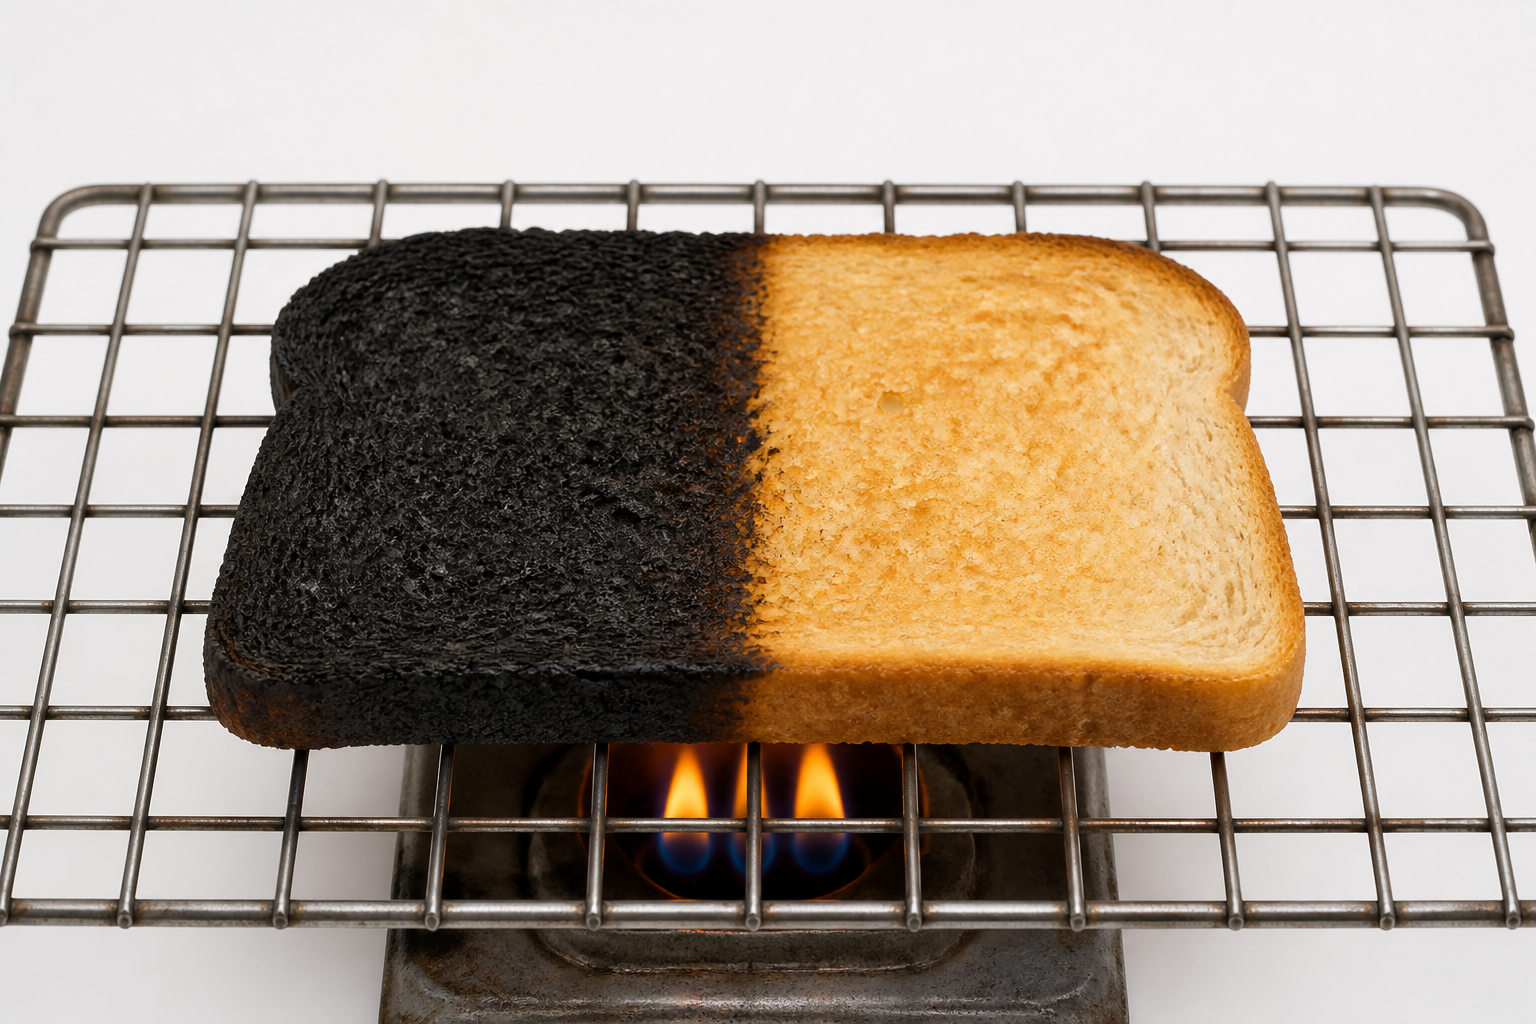
\includegraphics[width=0.6\linewidth]{images/book2/ai/g10-chem-charred-bread.png}

{\small Pão deixado tempo demais na grelha. O resíduo preto é quase só
carbono: as moléculas orgânicas do pão perderam o hidrogênio e o
oxigênio delas como vapor de água e gás carbônico, deixando para trás o
esqueleto de carbono.}
\end{omfigure}

\section{Exercícios}

\begin{exercise}[$\star$]\label{exo:g10:chemistry-of-life:1}
Cite os quatro elementos que formam 96\% da massa de um corpo vivo, com
as porcentagens aproximadas deles num ser humano.
\end{exercise}

\begin{exercise}[$\star$]\label{exo:g10:chemistry-of-life:2}
Classifique em \omterm{def:g10:chemistry-of-life:mineral-organic}{matéria mineral} e \omterm{def:g10:chemistry-of-life:mineral-organic}{matéria orgânica}: água, glicose,
cloreto de sódio, um triglicerídeo, fosfato de cálcio, um \omterm{def:g10:chemistry-of-life:families}{aminoácido},
gás carbônico.
\end{exercise}

\begin{exercise}[$\star$]\label{exo:g10:chemistry-of-life:3}
Uma folha de alface fresca de massa \qty{12.0}{g} é seca até massa
constante: \qty{0.6}{g}. Qual é o teor de água dela, em por cento?
\end{exercise}

\begin{exercise}[$\star$]\label{exo:g10:chemistry-of-life:4}
Que teste você usaria para mostrar que uma semente de feijão contém (a)
amido, (b) \omterm{def:g10:chemistry-of-life:families}{proteína}, (c) \omterm{def:g10:chemistry-of-life:families}{lipídios}? Dê o resultado esperado em cada caso.
\end{exercise}

\begin{exercise}[$\star$]\label{exo:g10:chemistry-of-life:5}
Dê o bloco de construção de cada família: \omterm{def:g10:chemistry-of-life:families}{carboidratos}, \omterm{def:g10:chemistry-of-life:families}{lipídios},
\omterm{def:g10:chemistry-of-life:families}{proteínas}, \omterm{def:g10:chemistry-of-life:families}{ácidos nucleicos}.
\end{exercise}

\begin{exercise}[$\star\star$]\label{exo:g10:chemistry-of-life:6}
Usando a primeira figura do capítulo, por que fator o carbono é mais
concentrado num corpo humano do que na crosta terrestre? E o
nitrogênio? Comente.
\end{exercise}

\begin{exercise}[$\star\star$]\label{exo:g10:chemistry-of-life:7}
Um adulto de massa \qty{70}{kg} é 62\% água. Calcule a massa de água do
corpo, depois a massa da matéria seca. Se as \omterm{def:g10:chemistry-of-life:families}{proteínas} são 17\% da
massa corporal, qual é a massa de \omterm{def:g10:chemistry-of-life:families}{proteína}?
\end{exercise}

\begin{exercise}[$\star\star$]\label{exo:g10:chemistry-of-life:8}
Uma barra de cereal contém, por \qty{100}{g}, \qty{60}{g} de
\omterm{def:g10:chemistry-of-life:families}{carboidratos}, \qty{12}{g} de \omterm{def:g10:chemistry-of-life:families}{lipídios} e \qty{8}{g} de \omterm{def:g10:chemistry-of-life:families}{proteínas}. Usando
os valores energéticos da \cref{prop:g10:chemistry-of-life:roles},
calcule a energia fornecida por \qty{100}{g} da barra, e a fração que
vem dos \omterm{def:g10:chemistry-of-life:families}{lipídios}.
\end{exercise}

\begin{exercise}[$\star\star$]\label{exo:g10:chemistry-of-life:9}
Adiciona-se solução de iodo a uma fatia de pão, a uma fatia de queijo e
a um torrão de açúcar. Preveja o resultado em cada caso e explique.
\end{exercise}

\begin{exercise}[$\star\star$]\label{exo:g10:chemistry-of-life:10}
Por que a matéria seca de uma planta queima, enquanto a cinza que ela
deixa não queima? De que família de matéria é cada uma?
\end{exercise}

\begin{exercise}[$\star\star$]\label{exo:g10:chemistry-of-life:11}
São dadas duas soluções: uma de glicose, outra de amido. O teste de
Fehling é positivo só para a primeira, o iodo só para a segunda. E no
entanto o amido é feito de glicose. Proponha uma explicação.
\end{exercise}

\begin{exercise}[$\star\star\star$]\label{exo:g10:chemistry-of-life:12}
Um grão de trigo contém 13\% de água; uma plântula de trigo três dias
depois da germinação contém 88\%. Explique a mudança, e o que ela diz a
você sobre o papel da água na química do grão.
\end{exercise}

\begin{exercise}[$\star\star\star$]\label{exo:g10:chemistry-of-life:13}
O plasma sanguíneo contém cerca de \qty{9}{g/L} de cloreto de sódio e
cerca de \qty{1}{g/L} de glicose. Um paciente recebe \qty{500}{mL} de
uma solução intravenosa. Que massas de sal e de glicose ela deve conter
para igualar o plasma? Por que a água pura seria perigosa?
\end{exercise}

\begin{exercise}[$\star\star\star$]\label{exo:g10:chemistry-of-life:14}
Os \omterm{def:g10:chemistry-of-life:families}{lipídios} armazenam \qty{38}{kJ/g}, o glicogênio \qty{17}{kJ/g}; além
disso cada grama de glicogênio do corpo é armazenada com cerca de
\qty{3}{g} de água. Uma pessoa carrega \qty{0.5}{kg} de glicogênio e
\qty{10}{kg} de \omterm{def:g10:chemistry-of-life:families}{lipídio}. Calcule a energia de cada reserva, e a massa
que um corpo precisaria carregar para guardar a energia da reserva de
\omterm{def:g10:chemistry-of-life:families}{lipídio} como glicogênio hidratado. Conclua sobre por que os animais
armazenam gordura.
\end{exercise}

\begin{exercise}[$\star\star\star$]\label{exo:g10:chemistry-of-life:15}
``Os seres vivos são feitos dos mesmos átomos que as rochas, logo não
há nada quimicamente especial na vida.'' Discuta essa afirmação num
parágrafo curto, usando três argumentos precisos do capítulo.
\end{exercise}

\section{Problema: o carbono de um ser humano}

\begin{problem}[{Problema de fim de semana --- de um campo de trigo a um
corpo: um balanço da matéria, da água de um grão ao número de quilogramas
de carbono que uma pessoa carrega}]
\label{pb:g10:chemistry-of-life:1}
Uma turma segue a matéria de um campo de trigo até o corpo de um dos
alunos dela. Dados: um grão de trigo é 13\% água, e a matéria seca dele
é cerca de 70\% amido, 12\% \omterm{def:g10:chemistry-of-life:families}{proteína}, 2\% \omterm{def:g10:chemistry-of-life:families}{lipídio}, 2\% mineral, o resto
celulose. A farinha de pão guarda aproximadamente a composição da parte
interna do grão. A aluna, Lea, tem massa de \qty{60}{kg}; use a
composição do adulto da segunda figura (água 60\%, \omterm{def:g10:chemistry-of-life:families}{proteínas} 17\%,
\omterm{def:g10:chemistry-of-life:families}{lipídios} 16\%, minerais 6\%, \omterm{def:g10:chemistry-of-life:families}{carboidratos} 1\%). Frações mássicas dos
elementos dentro de cada família: tome os \omterm{def:g10:chemistry-of-life:families}{carboidratos} como 40\%
carbono, os \omterm{def:g10:chemistry-of-life:families}{lipídios} como 77\% carbono, as \omterm{def:g10:chemistry-of-life:families}{proteínas} como 53\% carbono e
16\% nitrogênio.

\medskip
\noindent\textbf{Parte I --- O grão.}
\begin{enumerate}
  \item Um grão de massa \qty{45}{mg} é seco. Que massa de água ele
        perde, e qual é a massa seca dele?
  \item Calcule as massas de amido, \omterm{def:g10:chemistry-of-life:families}{proteína} e \omterm{def:g10:chemistry-of-life:families}{lipídio} na matéria seca
        de um grão.
  \item Que testes do \cref{met:g10:chemistry-of-life:tests}
        confirmariam cada um desses três constituintes num grão moído?
  \item O grão é plantado e regado; três dias depois a plântula é 88\%
        água. Explique por que a germinação não pode começar a 13\%.
  \item Um hectare rende \qty{8}{t} de grão. Que massa de água é
        colhida junto, e que massa de matéria seca?
\end{enumerate}

\medskip
\noindent\textbf{Parte II --- O pão.}
\begin{enumerate}[resume]
  \item Um pão é assado com \qty{500}{g} de farinha, \qty{320}{g} de
        água e \qty{10}{g} de sal; ele perde \qty{130}{g} de água no
        forno. Qual é a massa do pão assado, e o teor de água dele em
        por cento?
  \item Usando a composição seca do grão para a farinha, estime as
        massas de amido e de \omterm{def:g10:chemistry-of-life:families}{proteína} do pão.
  \item Usando \qty{17}{kJ/g} para \omterm{def:g10:chemistry-of-life:families}{carboidratos} e \omterm{def:g10:chemistry-of-life:families}{proteínas} e
        \qty{38}{kJ/g} para \omterm{def:g10:chemistry-of-life:families}{lipídios}, estime o conteúdo energético do
        pão.
  \item Lea come \qty{120}{g} desse pão. Que fração de uma necessidade
        diária de cerca de \qty{10000}{kJ} isso cobre?
  \item Por que o sal do pão não é uma fonte de energia, e para que ele
        serve no corpo?
\end{enumerate}

\medskip
\noindent\textbf{Parte III --- O corpo: a água e as famílias.}
\begin{enumerate}[resume]
  \item Calcule a massa de água do corpo de Lea.
  \item Calcule as massas de \omterm{def:g10:chemistry-of-life:families}{proteína}, de \omterm{def:g10:chemistry-of-life:families}{lipídio}, de mineral e de
        \omterm{def:g10:chemistry-of-life:families}{carboidrato}.
  \item Lea perde \qty{1.2}{kg} por transpiração durante uma corrida
        longa. Que fração da água do corpo dela é isso? Por que isso
        precisa ser reposto depressa?
  \item O sangue dela, cerca de \qty{4.5}{L}, é 55\% plasma, e o plasma
        é 90\% água. Estime a massa de água do sangue dela (tome
        \qty{1}{kg} por litro). Que fração da água do corpo dela é
        isso? Onde está o resto?
  \item Um recém-nascido é 75\% água. Explique numa frase por que um
        bebê é mais vulnerável à desidratação do que um adulto.
\end{enumerate}

\medskip
\noindent\textbf{Parte IV --- O corpo: os elementos.}
\begin{enumerate}[resume]
  \item Usando as frações de carbono de cada família, calcule a massa
        de carbono dos \omterm{def:g10:chemistry-of-life:families}{carboidratos}, dos \omterm{def:g10:chemistry-of-life:families}{lipídios} e das \omterm{def:g10:chemistry-of-life:families}{proteínas} de
        Lea, depois a massa total de carbono.
  \item Que fração da massa corporal dela é carbono? Compare com os
        18.5\% da \cref{prop:g10:chemistry-of-life:four} e comente a
        concordância.
  \item Calcule a massa de nitrogênio das \omterm{def:g10:chemistry-of-life:families}{proteínas} dela. De onde veio,
        no fim das contas, esse nitrogênio?
  \item A água é 89\% oxigênio em massa. Calcule a massa de oxigênio
        carregada só pela água do corpo dela, e compare com os 65\% da
        \cref{prop:g10:chemistry-of-life:four}. Que molécula explica a
        maior parte do oxigênio do corpo?
  \item Enuncie o resultado numa frase: quantos quilogramas de carbono
        uma pessoa de \qty{60}{kg} carrega, e por quais dois processos
        biológicos esse carbono deixou o ar e entrou no corpo?
\end{enumerate}
\end{problem}
